\documentclass{standalone}
\usepackage{tikz}
\usetikzlibrary{patterns, positioning}


\begin{document}
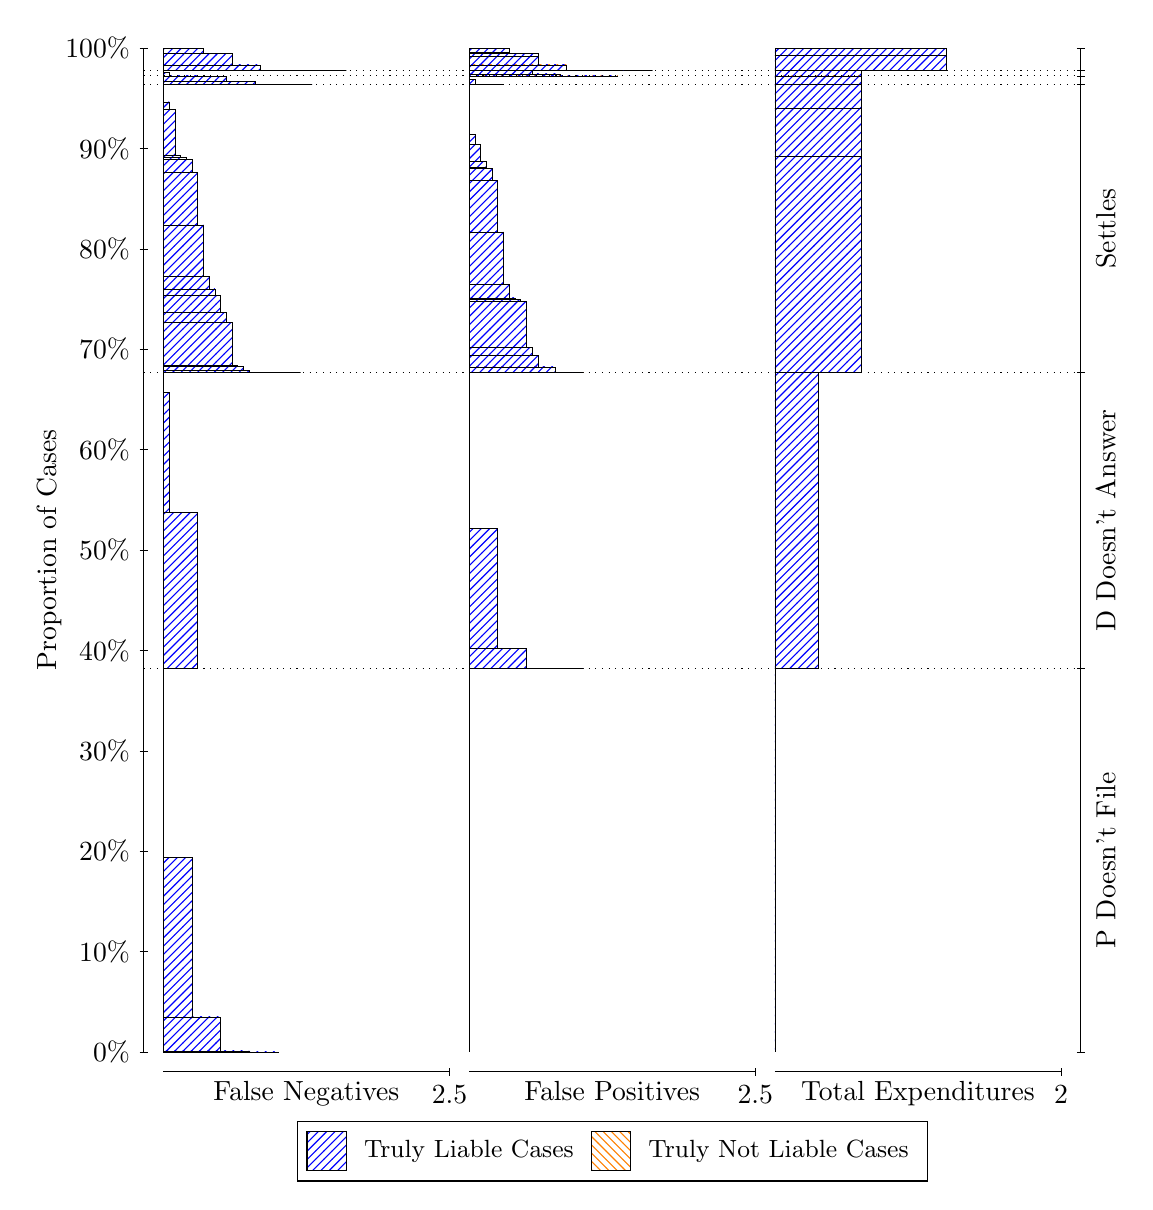
\begin{tikzpicture}
\draw[black, very thin] (1.5,1.75) -- (1.5,14.5);
\node[rotate=90, text=black, anchor=center] at (0.3, 8.125) {Proportion of Cases};
\draw[black, very thin] (1.45,1.75) -- (1.55,1.75);
\node[text=black, anchor=east] at (1.45, 1.75) {0\%};
\draw[black, very thin] (1.45,3.025) -- (1.55,3.025);
\node[text=black, anchor=east] at (1.45, 3.025) {10\%};
\draw[black, very thin] (1.45,4.3) -- (1.55,4.3);
\node[text=black, anchor=east] at (1.45, 4.3) {20\%};
\draw[black, very thin] (1.45,5.575) -- (1.55,5.575);
\node[text=black, anchor=east] at (1.45, 5.575) {30\%};
\draw[black, very thin] (1.45,6.85) -- (1.55,6.85);
\node[text=black, anchor=east] at (1.45, 6.85) {40\%};
\draw[black, very thin] (1.45,8.125) -- (1.55,8.125);
\node[text=black, anchor=east] at (1.45, 8.125) {50\%};
\draw[black, very thin] (1.45,9.4) -- (1.55,9.4);
\node[text=black, anchor=east] at (1.45, 9.4) {60\%};
\draw[black, very thin] (1.45,10.675) -- (1.55,10.675);
\node[text=black, anchor=east] at (1.45, 10.675) {70\%};
\draw[black, very thin] (1.45,11.95) -- (1.55,11.95);
\node[text=black, anchor=east] at (1.45, 11.95) {80\%};
\draw[black, very thin] (1.45,13.225) -- (1.55,13.225);
\node[text=black, anchor=east] at (1.45, 13.225) {90\%};
\draw[black, very thin] (1.45,14.5) -- (1.55,14.5);
\node[text=black, anchor=east] at (1.45, 14.5) {100\%};

\draw[black, very thin] (13.4,1.75) -- (13.4,14.5);
\draw[black, very thin] (13.35,1.75) -- (13.45,1.75);
\node[anchor=west] at (13.35, 1.75) {};
\draw[black, very thin] (13.35,6.6223) -- (13.45,6.6223);
\node[anchor=west] at (13.35, 6.6223) {};
\draw[black, very thin] (13.35,10.377) -- (13.45,10.377);
\node[anchor=west] at (13.35, 10.377) {};
\draw[black, very thin] (13.35,14.04) -- (13.45,14.04);
\node[anchor=west] at (13.35, 14.04) {};
\draw[black, very thin] (13.35,14.146) -- (13.45,14.146);
\node[anchor=west] at (13.35, 14.146) {};
\draw[black, very thin] (13.35,14.215) -- (13.45,14.215);
\node[anchor=west] at (13.35, 14.215) {};
\draw[black, very thin] (13.35,14.5) -- (13.45,14.5);
\node[anchor=west] at (13.35, 14.5) {};

\draw[black, very thin, pattern color=blue, pattern=north east lines] (1.75,1.75) rectangle (3.2033,1.7501);
\draw[black, very thin, pattern color=blue, pattern=north east lines] (1.75,1.7501) rectangle (2.84,1.7649);
\draw[black, very thin, pattern color=blue, pattern=north east lines] (1.75,1.7649) rectangle (2.4767,2.1957);
\draw[black, very thin, pattern color=blue, pattern=north east lines] (1.75,2.1957) rectangle (2.1133,4.226);
\draw[black, very thin, pattern color=orange, pattern=north west lines] (1.75,4.226) rectangle (1.75,4.226);
\draw[black, very thin, pattern color=blue, pattern=north east lines] (1.75,4.226) rectangle (1.75,6.6223);
\draw[black, very thin, pattern color=blue, pattern=north east lines] (1.75,6.6223) rectangle (2.186,8.6023);
\draw[black, very thin, pattern color=blue, pattern=north east lines] (1.75,8.6023) rectangle (1.8227,10.128);
\draw[black, very thin, pattern color=orange, pattern=north west lines] (1.75,10.128) rectangle (1.75,10.128);
\draw[black, very thin, pattern color=blue, pattern=north east lines] (1.75,10.128) rectangle (1.75,10.377);
\draw[black, very thin, pattern color=blue, pattern=north east lines] (1.75,10.377) rectangle (3.494,10.377);
\draw[black, very thin, pattern color=blue, pattern=north east lines] (1.75,10.377) rectangle (3.2033,10.377);
\draw[black, very thin, pattern color=blue, pattern=north east lines] (1.75,10.377) rectangle (3.1307,10.378);
\draw[black, very thin, pattern color=blue, pattern=north east lines] (1.75,10.378) rectangle (3.058,10.378);
\draw[black, very thin, pattern color=blue, pattern=north east lines] (1.75,10.378) rectangle (2.9127,10.379);
\draw[black, very thin, pattern color=blue, pattern=north east lines] (1.75,10.379) rectangle (2.84,10.407);
\draw[black, very thin, pattern color=blue, pattern=north east lines] (1.75,10.407) rectangle (2.7673,10.46);
\draw[black, very thin, pattern color=blue, pattern=north east lines] (1.75,10.46) rectangle (2.6947,10.467);
\draw[black, very thin, pattern color=blue, pattern=north east lines] (1.75,10.467) rectangle (2.622,11.015);
\draw[black, very thin, pattern color=blue, pattern=north east lines] (1.75,11.015) rectangle (2.5493,11.138);
\draw[black, very thin, pattern color=blue, pattern=north east lines] (1.75,11.138) rectangle (2.4767,11.354);
\draw[black, very thin, pattern color=blue, pattern=north east lines] (1.75,11.354) rectangle (2.404,11.43);
\draw[black, very thin, pattern color=blue, pattern=north east lines] (1.75,11.43) rectangle (2.404,11.442);
\draw[black, very thin, pattern color=blue, pattern=north east lines] (1.75,11.442) rectangle (2.3313,11.598);
\draw[black, very thin, pattern color=blue, pattern=north east lines] (1.75,11.598) rectangle (2.2587,12.253);
\draw[black, very thin, pattern color=blue, pattern=north east lines] (1.75,12.253) rectangle (2.186,12.924);
\draw[black, very thin, pattern color=blue, pattern=north east lines] (1.75,12.924) rectangle (2.1133,13.089);
\draw[black, very thin, pattern color=blue, pattern=north east lines] (1.75,13.089) rectangle (2.0407,13.108);
\draw[black, very thin, pattern color=blue, pattern=north east lines] (1.75,13.108) rectangle (2.0407,13.108);
\draw[black, very thin, pattern color=blue, pattern=north east lines] (1.75,13.108) rectangle (1.968,13.135);
\draw[black, very thin, pattern color=blue, pattern=north east lines] (1.75,13.135) rectangle (1.8953,13.716);
\draw[black, very thin, pattern color=blue, pattern=north east lines] (1.75,13.716) rectangle (1.8227,13.817);
\draw[black, very thin, pattern color=orange, pattern=north west lines] (1.75,13.817) rectangle (1.75,13.817);
\draw[black, very thin, pattern color=blue, pattern=north east lines] (1.75,13.817) rectangle (1.75,14.04);
\draw[black, very thin, pattern color=blue, pattern=north east lines] (1.75,14.04) rectangle (3.6393,14.04);
\draw[black, very thin, pattern color=blue, pattern=north east lines] (1.75,14.04) rectangle (3.276,14.04);
\draw[black, very thin, pattern color=blue, pattern=north east lines] (1.75,14.04) rectangle (2.9127,14.08);
\draw[black, very thin, pattern color=blue, pattern=north east lines] (1.75,14.08) rectangle (2.5493,14.144);
\draw[black, very thin, pattern color=blue, pattern=north east lines] (1.75,14.144) rectangle (2.186,14.146);
\draw[black, very thin, pattern color=orange, pattern=north west lines] (1.75,14.146) rectangle (1.75,14.146);
\draw[black, very thin, pattern color=blue, pattern=north east lines] (1.75,14.146) rectangle (2.186,14.147);
\draw[black, very thin, pattern color=blue, pattern=north east lines] (1.75,14.147) rectangle (1.8227,14.189);
\draw[black, very thin, pattern color=orange, pattern=north west lines] (1.75,14.189) rectangle (1.75,14.189);
\draw[black, very thin, pattern color=blue, pattern=north east lines] (1.75,14.189) rectangle (1.75,14.215);
\draw[black, very thin, pattern color=blue, pattern=north east lines] (1.75,14.215) rectangle (4.0753,14.215);
\draw[black, very thin, pattern color=blue, pattern=north east lines] (1.75,14.215) rectangle (3.712,14.215);
\draw[black, very thin, pattern color=blue, pattern=north east lines] (1.75,14.215) rectangle (3.3487,14.22);
\draw[black, very thin, pattern color=blue, pattern=north east lines] (1.75,14.22) rectangle (2.9853,14.286);
\draw[black, very thin, pattern color=blue, pattern=north east lines] (1.75,14.286) rectangle (2.622,14.429);
\draw[black, very thin, pattern color=blue, pattern=north east lines] (1.75,14.429) rectangle (2.2587,14.495);
\draw[black, very thin, pattern color=blue, pattern=north east lines] (1.75,14.495) rectangle (1.8953,14.5);
\draw[black, very thin, pattern color=orange, pattern=north west lines] (1.75,14.5) rectangle (1.75,14.5);
\draw[black, very thin, pattern color=blue, pattern=north east lines] (1.75,14.5) rectangle (1.75,14.5);
\draw[black, very thin, pattern color=orange, pattern=north west lines] (5.6333,1.75) rectangle (5.6333,1.75);
\draw[black, very thin, pattern color=blue, pattern=north east lines] (5.6333,1.75) rectangle (5.6333,6.6223);
\draw[black, very thin, pattern color=orange, pattern=north west lines] (5.6333,6.6223) rectangle (7.0867,6.6223);
\draw[black, very thin, pattern color=blue, pattern=north east lines] (5.6333,6.6223) rectangle (7.0867,6.6223);
\draw[black, very thin, pattern color=blue, pattern=north east lines] (5.6333,6.6223) rectangle (6.7233,6.6234);
\draw[black, very thin, pattern color=blue, pattern=north east lines] (5.6333,6.6234) rectangle (6.36,6.8713);
\draw[black, very thin, pattern color=blue, pattern=north east lines] (5.6333,6.8713) rectangle (5.9967,8.3969);
\draw[black, very thin, pattern color=blue, pattern=north east lines] (5.6333,8.3969) rectangle (5.6333,10.377);
\draw[black, very thin, pattern color=orange, pattern=north west lines] (5.6333,10.377) rectangle (7.0867,10.377);
\draw[black, very thin, pattern color=blue, pattern=north east lines] (5.6333,10.377) rectangle (7.0867,10.377);
\draw[black, very thin, pattern color=orange, pattern=north west lines] (5.6333,10.377) rectangle (6.9413,10.377);
\draw[black, very thin, pattern color=blue, pattern=north east lines] (5.6333,10.377) rectangle (6.9413,10.377);
\draw[black, very thin, pattern color=orange, pattern=north west lines] (5.6333,10.377) rectangle (6.796,10.377);
\draw[black, very thin, pattern color=blue, pattern=north east lines] (5.6333,10.377) rectangle (6.796,10.377);
\draw[black, very thin, pattern color=blue, pattern=north east lines] (5.6333,10.377) rectangle (6.7233,10.45);
\draw[black, very thin, pattern color=orange, pattern=north west lines] (5.6333,10.45) rectangle (6.6507,10.45);
\draw[black, very thin, pattern color=blue, pattern=north east lines] (5.6333,10.45) rectangle (6.6507,10.45);
\draw[black, very thin, pattern color=blue, pattern=north east lines] (5.6333,10.45) rectangle (6.578,10.45);
\draw[black, very thin, pattern color=orange, pattern=north west lines] (5.6333,10.45) rectangle (6.5053,10.45);
\draw[black, very thin, pattern color=blue, pattern=north east lines] (5.6333,10.45) rectangle (6.5053,10.6);
\draw[black, very thin, pattern color=blue, pattern=north east lines] (5.6333,10.6) rectangle (6.4327,10.701);
\draw[black, very thin, pattern color=blue, pattern=north east lines] (5.6333,10.701) rectangle (6.36,11.282);
\draw[black, very thin, pattern color=blue, pattern=north east lines] (5.6333,11.282) rectangle (6.2873,11.309);
\draw[black, very thin, pattern color=orange, pattern=north west lines] (5.6333,11.309) rectangle (6.2147,11.309);
\draw[black, very thin, pattern color=blue, pattern=north east lines] (5.6333,11.309) rectangle (6.2147,11.309);
\draw[black, very thin, pattern color=blue, pattern=north east lines] (5.6333,11.309) rectangle (6.2147,11.328);
\draw[black, very thin, pattern color=blue, pattern=north east lines] (5.6333,11.328) rectangle (6.142,11.494);
\draw[black, very thin, pattern color=blue, pattern=north east lines] (5.6333,11.494) rectangle (6.0693,12.164);
\draw[black, very thin, pattern color=blue, pattern=north east lines] (5.6333,12.164) rectangle (5.9967,12.819);
\draw[black, very thin, pattern color=blue, pattern=north east lines] (5.6333,12.819) rectangle (5.924,12.975);
\draw[black, very thin, pattern color=blue, pattern=north east lines] (5.6333,12.975) rectangle (5.8513,12.987);
\draw[black, very thin, pattern color=blue, pattern=north east lines] (5.6333,12.987) rectangle (5.8513,13.063);
\draw[black, very thin, pattern color=blue, pattern=north east lines] (5.6333,13.063) rectangle (5.7787,13.279);
\draw[black, very thin, pattern color=blue, pattern=north east lines] (5.6333,13.279) rectangle (5.706,13.402);
\draw[black, very thin, pattern color=blue, pattern=north east lines] (5.6333,13.402) rectangle (5.6333,14.04);
\draw[black, very thin, pattern color=orange, pattern=north west lines] (5.6333,14.04) rectangle (6.0693,14.04);
\draw[black, very thin, pattern color=blue, pattern=north east lines] (5.6333,14.04) rectangle (6.0693,14.042);
\draw[black, very thin, pattern color=blue, pattern=north east lines] (5.6333,14.042) rectangle (5.706,14.106);
\draw[black, very thin, pattern color=blue, pattern=north east lines] (5.6333,14.106) rectangle (5.6333,14.146);
\draw[black, very thin, pattern color=orange, pattern=north west lines] (5.6333,14.146) rectangle (7.5227,14.146);
\draw[black, very thin, pattern color=blue, pattern=north east lines] (5.6333,14.146) rectangle (7.5227,14.146);
\draw[black, very thin, pattern color=blue, pattern=north east lines] (5.6333,14.146) rectangle (7.1593,14.146);
\draw[black, very thin, pattern color=blue, pattern=north east lines] (5.6333,14.146) rectangle (6.796,14.172);
\draw[black, very thin, pattern color=blue, pattern=north east lines] (5.6333,14.172) rectangle (6.4327,14.214);
\draw[black, very thin, pattern color=blue, pattern=north east lines] (5.6333,14.214) rectangle (6.0693,14.215);
\draw[black, very thin, pattern color=orange, pattern=north west lines] (5.6333,14.215) rectangle (7.9587,14.215);
\draw[black, very thin, pattern color=blue, pattern=north east lines] (5.6333,14.215) rectangle (7.9587,14.215);
\draw[black, very thin, pattern color=orange, pattern=north west lines] (5.6333,14.215) rectangle (7.5953,14.215);
\draw[black, very thin, pattern color=blue, pattern=north east lines] (5.6333,14.215) rectangle (7.5953,14.215);
\draw[black, very thin, pattern color=orange, pattern=north west lines] (5.6333,14.215) rectangle (7.232,14.215);
\draw[black, very thin, pattern color=blue, pattern=north east lines] (5.6333,14.215) rectangle (7.232,14.22);
\draw[black, very thin, pattern color=blue, pattern=north east lines] (5.6333,14.22) rectangle (6.8687,14.286);
\draw[black, very thin, pattern color=orange, pattern=north west lines] (5.6333,14.286) rectangle (6.8687,14.286);
\draw[black, very thin, pattern color=blue, pattern=north east lines] (5.6333,14.286) rectangle (6.8687,14.286);
\draw[black, very thin, pattern color=blue, pattern=north east lines] (5.6333,14.286) rectangle (6.5053,14.39);
\draw[black, very thin, pattern color=orange, pattern=north west lines] (5.6333,14.39) rectangle (6.5053,14.39);
\draw[black, very thin, pattern color=blue, pattern=north east lines] (5.6333,14.39) rectangle (6.5053,14.429);
\draw[black, very thin, pattern color=blue, pattern=north east lines] (5.6333,14.429) rectangle (6.142,14.447);
\draw[black, very thin, pattern color=blue, pattern=north east lines] (5.6333,14.447) rectangle (6.142,14.495);
\draw[black, very thin, pattern color=blue, pattern=north east lines] (5.6333,14.495) rectangle (5.7787,14.495);
\draw[black, very thin, pattern color=blue, pattern=north east lines] (5.6333,14.495) rectangle (5.7787,14.5);
\draw[black, very thin, pattern color=blue, pattern=north east lines] (5.6333,14.5) rectangle (5.6333,14.5);
\draw[black, very thin, pattern color=orange, pattern=north west lines] (9.5167,1.75) rectangle (9.5167,1.75);
\draw[black, very thin, pattern color=blue, pattern=north east lines] (9.5167,1.75) rectangle (9.5167,6.6223);
\draw[black, very thin, pattern color=orange, pattern=north west lines] (9.5167,6.6223) rectangle (10.062,6.6223);
\draw[black, very thin, pattern color=blue, pattern=north east lines] (9.5167,6.6223) rectangle (10.062,10.377);
\draw[black, very thin, pattern color=orange, pattern=north west lines] (9.5167,10.377) rectangle (10.607,10.377);
\draw[black, very thin, pattern color=blue, pattern=north east lines] (9.5167,10.377) rectangle (10.607,13.128);
\draw[black, very thin, pattern color=orange, pattern=north west lines] (9.5167,13.128) rectangle (10.607,13.128);
\draw[black, very thin, pattern color=blue, pattern=north east lines] (9.5167,13.128) rectangle (10.607,13.735);
\draw[black, very thin, pattern color=orange, pattern=north west lines] (9.5167,13.735) rectangle (10.607,13.735);
\draw[black, very thin, pattern color=blue, pattern=north east lines] (9.5167,13.735) rectangle (10.607,14.04);
\draw[black, very thin, pattern color=orange, pattern=north west lines] (9.5167,14.04) rectangle (10.607,14.04);
\draw[black, very thin, pattern color=blue, pattern=north east lines] (9.5167,14.04) rectangle (10.607,14.146);
\draw[black, very thin, pattern color=orange, pattern=north west lines] (9.5167,14.146) rectangle (10.607,14.146);
\draw[black, very thin, pattern color=blue, pattern=north east lines] (9.5167,14.146) rectangle (10.607,14.215);
\draw[black, very thin, pattern color=orange, pattern=north west lines] (9.5167,14.215) rectangle (11.697,14.215);
\draw[black, very thin, pattern color=blue, pattern=north east lines] (9.5167,14.215) rectangle (11.697,14.407);
\draw[black, very thin, pattern color=orange, pattern=north west lines] (9.5167,14.407) rectangle (11.697,14.407);
\draw[black, very thin, pattern color=blue, pattern=north east lines] (9.5167,14.407) rectangle (11.697,14.5);
\draw[black, dotted] (1.5,6.6223) -- (13.4,6.6223);
\draw[black, dotted] (1.5,10.377) -- (13.4,10.377);
\draw[black, dotted] (1.5,14.04) -- (13.4,14.04);
\draw[black, dotted] (1.5,14.146) -- (13.4,14.146);
\draw[black, dotted] (1.5,14.215) -- (13.4,14.215);
\draw[black, very thin] (1.75,1.5) -- (5.3833,1.5);
\node[text=black, anchor=north] at (3.5667, 1.5) {False Negatives};
\draw[black, very thin] (5.3833,1.45) -- (5.3833,1.55);
\node[text=black, anchor=north] at (5.3833, 1.45) {2.5};

\draw[black, very thin] (5.6333,1.5) -- (9.2667,1.5);
\node[text=black, anchor=north] at (7.45, 1.5) {False Positives};
\draw[black, very thin] (9.2667,1.45) -- (9.2667,1.55);
\node[text=black, anchor=north] at (9.2667, 1.45) {2.5};

\draw[black, very thin] (9.5167,1.5) -- (13.15,1.5);
\node[text=black, anchor=north] at (11.333, 1.5) {Total Expenditures};
\draw[black, very thin] (13.15,1.45) -- (13.15,1.55);
\node[text=black, anchor=north] at (13.15, 1.45) {2};

\node[text=black, centered, rotate=90] at (13.72, 4.1861) {P Doesn't File};
\node[text=black, centered, rotate=90] at (13.72, 8.4996) {D Doesn't Answer};
\node[text=black, centered, rotate=90] at (13.72, 12.209) {Settles};




\draw (7.449999999999999,1.5) node[draw=none] (baseCoordinate) {};
\begin{scope}[align=center]
        \matrix[scale=0.5, draw=black, below=0.5cm of baseCoordinate, nodes={draw}, column sep=0.1cm]{
            \node[rectangle, draw, minimum width=0.5cm, minimum height=0.5cm, pattern color=blue, pattern=north east lines] {}; &
            \node[draw=none, font=\small, text=black] (B) {Truly Liable Cases}; &
            \node[rectangle, draw, minimum width=0.5cm, minimum height=0.5cm, pattern color=orange, pattern=north west lines] {}; &
            \node[draw=none, font=\small, text=black] (B) {Truly Not Liable Cases}; \\
            };
\end{scope}

\end{tikzpicture}
\end{document}